\documentclass[12pt]{article}

%%%%%%%%%%%%%%%%%%%%%%%%%%%%%%%%%%%%%%%%%%%%%%%%%%%%%%%%%%%%%%%%%%%%%%%%%%%%%%%%
%                           Package preset for homework
%%%%%%%%%%%%%%%%%%%%%%%%%%%%%%%%%%%%%%%%%%%%%%%%%%%%%%%%%%%%%%%%%%%%%%%%%%%%%%%%
% Miscellaneous
\usepackage[margin=1in]{geometry}
\usepackage[utf8]{inputenc}
\usepackage{indentfirst}
\usepackage{blindtext}
\usepackage{graphicx}
\usepackage{xr-hyper}
\usepackage{hyperref}
\usepackage{enumitem}
\usepackage{color}
\usepackage{float}
% Math
\usepackage{latexsym}
\usepackage{amsfonts}
\usepackage{amssymb}
\usepackage{amsmath}
\usepackage{commath}
\usepackage{amsthm}
\usepackage{bbold}
\usepackage{bm}
% Physics
\usepackage{physics}
\usepackage{siunitx}
% Code typesetting
\usepackage{listings}
% Citation
\usepackage[authoryear]{natbib}
\usepackage{appendix}
\usepackage[capitalize]{cleveref}
% Title & name
\title{Homework}
\author{Tien Vo}
\date{\today}


%%%%%%%%%%%%%%%%%%%%%%%%%%%%%%%%%%%%%%%%%%%%%%%%%%%%%%%%%%%%%%%%%%%%%%%%%%%%%%%%
%                   User-defined commands and environments
%%%%%%%%%%%%%%%%%%%%%%%%%%%%%%%%%%%%%%%%%%%%%%%%%%%%%%%%%%%%%%%%%%%%%%%%%%%%%%%%
%%% Misc
\sisetup{load-configurations=abbreviations}
\newcommand{\due}[1]{\date{Due: #1}}
\newcommand{\hint}{\textit{Hint}}
\let\oldt\t
\renewcommand{\t}[1]{\text{#1}}

%%% Bold sets & abbrv
\newcommand{\N}{\mathbb{N}}
\newcommand{\Z}{\mathbb{Z}}
\newcommand{\R}{\mathbb{R}}
\newcommand{\Q}{\mathbb{Q}}
\let\oldP\P
\renewcommand{\P}{\mathbb{P}}
\newcommand{\LL}{\mathcal{L}}
\newcommand{\FF}{\mathcal{F}}
\newcommand{\HH}{\mathcal{H}}
\newcommand{\NN}{\mathcal{N}}
\newcommand{\ZZ}{\mathcal{Z}}
\newcommand{\RN}[1]{\textup{\uppercase\expandafter{\romannumeral#1}}}
\newcommand{\ua}{\uparrow}
\newcommand{\da}{\downarrow}

%%% Unit vectors
\newcommand{\xhat}{\vb{\hat{x}}}
\newcommand{\yhat}{\vb{\hat{y}}}
\newcommand{\zhat}{\vb{\hat{z}}}
\newcommand{\nhat}{\vb{\hat{n}}}
\newcommand{\rhat}{\vb{\hat{r}}}
\newcommand{\phihat}{\bm{\hat{\phi}}}
\newcommand{\thetahat}{\bm{\hat{\theta}}}

%%% Other math stuff
\providecommand{\units}[1]{\,\ensuremath{\mathrm{#1}}\xspace}
% Set new style for problem
\newtheoremstyle{problemstyle}  % <name>
        {10pt}                   % <space above>
        {10pt}                   % <space below>
        {\normalfont}           % <body font>
        {}                      % <indent amount}
        {\bfseries\itshape}     % <theorem head font>
        {\normalfont\bfseries:} % <punctuation after theorem head>
        {.5em}                  % <space after theorem head>
        {}                      % <theorem head spec (can be left empty, 
                                % meaning `normal')>

% Set problem environment
\theoremstyle{problemstyle}
\newtheorem{problemenv}{Problem}[section]
\newenvironment{problem}[1]{%
  \renewcommand\theproblemenv{#1}%
  \problemenv
}{\endproblemenv}
% Set lemma environment
\newenvironment{lemma}[2][Lemma]{\begin{trivlist}
\item[\hskip \labelsep {\bfseries #1}\hskip \labelsep {\bfseries #2.}]}{\end{trivlist}}
% Set solution environment
\newenvironment{solution}{
    \begin{proof}[Solution]$ $\par\nobreak\ignorespaces
}{\end{proof}}
\numberwithin{equation}{problemenv}

%%% Page format
\setlength{\parindent}{0.5cm}
\setlength{\oddsidemargin}{0in}
\setlength{\textwidth}{6.5in}
\setlength{\textheight}{8.8in}
\setlength{\topmargin}{0in}
\setlength{\headheight}{18pt}

%%% Code environments
\definecolor{dkgreen}{rgb}{0,0.6,0}
\definecolor{gray}{rgb}{0.5,0.5,0.5}
\definecolor{mauve}{rgb}{0.58,0,0.82}
\lstset{frame=tb,
  language=Python,
  aboveskip=3mm,
  belowskip=3mm,
  showstringspaces=false,
  columns=flexible,
  basicstyle={\small\ttfamily},
  numbers=none,
  numberstyle=\tiny\color{gray},
  keywordstyle=\color{blue},
  commentstyle=\color{dkgreen},
  stringstyle=\color{mauve},
  breaklines=true,
  breakatwhitespace=true,
  tabsize=4
}
\lstset{
  language=Mathematica,
  numbers=left,
  numberstyle=\tiny\color{gray},
  numbersep=5pt,
  breaklines=true,
  captionpos={t},
  frame={lines},
  rulecolor=\color{black},
  framerule=0.5pt,
  columns=flexible,
  tabsize=2
}


\title{Homework 7: Phys 5210 (Fall 2021)}

\begin{document}
\maketitle
%%%%%%%%%%%%%%%%%%%%%%%%%%%%%%%%%%%%%%%%%%%%%%%%%%%%%%%%%%%%%%%%%%%%%%%%%%%%%%%%
\begin{problem}{1}
At the bowling alley a bowling ball (a solid uniform sphere of radius $R$ and
mass $m$) was thrown horzontally without spinning with the horizontal velocity
$v_0$. It hit the floor and, thanks to the friction between the ball and the
floor, eventually started rolling along without slipping. Find its final
velocity $v$. Neglect air resistance and the rolling friction (so that once it
starts rolling without slipping, there's no friction). Which fraction of the
initial kinetic energy of the ball was converted into heat during this process?
\begin{solution}
Assume that the frictional force $F$ is constant when the ball starts rolling. 
The time it takes to accelerate from $\omega_i=0$ to $\omega_f=\omega$
is
\begin{equation}
    t=\frac{\omega}{\alpha}=\frac{\omega I}{F R}
\end{equation}
where $\alpha =FR / I$ is the angular acceleration and $I=(2 /5)mR^2$ is the
moment of inertia of a uniform sphere of mass $m$ and radius $R$. In this
period, the linear velocity is decelerated to
\begin{equation}
    v=v_0-at=v_0-\frac{a}{F}\frac{\omega I}{R}=v_0-\frac25\omega R=v_0-\frac25v 
    \Rightarrow v=\frac57v_0
\end{equation}
Then we can calculate the fractional energy loss as
\begin{equation}
    \overline{W}=\frac{E_i-E_f}{E_i}=1-\frac{1 /2mv_0^2}{1/2mv^2+1/2I\omega^2} 
    =\frac{49/50mv^2}{7/10mv^2}=\frac27
\end{equation}
where we have written $\omega=vR$ since it starts rolling without slipping.
\end{solution}
\end{problem}
%%%%%%%%%%%%%%%%%%%%%%%%%%%%%%%%%%%%%%%%%%%%%%%%%%%%%%%%%%%%%%%%%%%%%%%%%%%%%%%%    
%%%%%%%%%%%%%%%%%%%%%%%%%%%%%%%%%%%%%%%%%%%%%%%%%%%%%%%%%%%%%%%%%%%%%%%%%%%%%%%%
\begin{problem}{2}[Goldstein, Problem 5.24]
A wheel rolls down a flat inclined surface that makes an angle $\alpha$ with the
horizontal (without slipping). The wheel is constrained so that its plane is
always perpendicular to the inclined plane, but it may rotate about the axis
normal to the surface. Think of a wheel as a symmetric top, with the moment of
inertia $I_3$ defined with respect to the axis perpendicular to the plane of the
wheel, and the two other moments of inertia $I_1=I_2\neq I_3$. Suppose the wheel
starts moving from rest.

Reduce its equations of motion to a single second order differential equation
the function $\phi(t)$ satisfies, where $\phi$ is the azimuthal angle describing
the direction where the wheel is rolling. Use the Lagrange function with the
appropriate Lagrange multipliers.
\begin{solution}
\begin{center}
    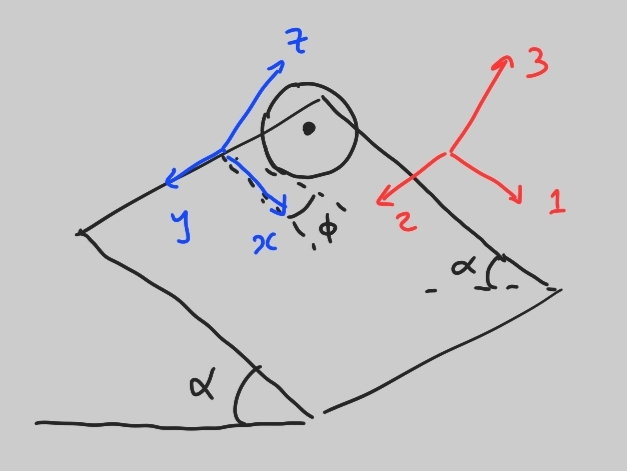
\includegraphics[width=0.5\textwidth]{hw7_p2.jpg} 
\end{center} 
Define our coordinate system as above. By definition, the angular velocity
around the principal axes of the wheel is
\begin{equation}
    \Omega_1=\dot\phi\sin\psi,\qquad
    \Omega_2=-\dot\phi\cos\psi,\qquad\text{and}\qquad
    \Omega_3=\dot\psi
\end{equation}
if we are to impose the constraint that the wheel is always perpendicular to the
plane of the ramp $(\theta=\pi /2)$. Because the wheel rolls without slipping,
the following constraints must be applied
\begin{equation}\label{p2:xydot}
    \dot{x}=R\cos\phi\dot\psi\qquad\text{and}\qquad
    \dot{y}=R\sin\phi\dot\psi
\end{equation}
Then we can write the Lagrange function (with Lagrange multipliers) as
\begin{align}
    \LL&=\frac12m(\dot{x}^2+\dot{y}^2)+\frac12I_1(\Omega_1^2+\Omega_2^2)+\frac12I_3\Omega_3^2+mgx\sin\alpha-\lambda_1(\dot{x}-R\cos\phi\dot\psi)-\lambda_2(\dot{y}-R\sin\phi\dot\psi)\notag\\
       &=\frac12m(\dot{x}^2+\dot{y}^2)+\frac14mR^2\dot\phi^2+\frac12mR^2\dot\psi^2+mgx\sin\alpha-\lambda_1(\dot{x}-R\cos\phi\dot\psi)-\lambda_2(\dot{y}-R\sin\phi\dot\psi)
\end{align}
where $I_1=I_2=1 /2I_3=1 /2mR^2$ are the moments of inertia of the wheel. Applying 
Euler-Lagrange equations for $x$ and $y$, we can write
\begin{subequations}
    \begin{align}
        m\ddot{x}&=mg\sin\alpha\\
        m\ddot{y}&=0
    \end{align} 
\end{subequations}
These are forces acting on the center of mass of the wheel, as expected
from Newtonian mechanics. From \eqref{p2:xydot}, it follows that
\begin{subequations}
    \begin{align}
        \qty(R\cos\phi)\ddot\psi-\qty(R\sin\phi)\dot{\phi}\dot\psi&=g\sin\alpha\\
        \qty(R\sin\phi)\ddot\psi+\qty(R\cos\phi)\dot\phi\dot\psi&=0
    \end{align} 
\end{subequations}
We can then solve this system for
\begin{equation}\label{p2:psidot}
    \dot\psi=-\frac{g\sin\alpha\sin\phi}{R\dot{\phi}}
    \qquad\text{and}\qquad
    \ddot\psi=\frac{g\sin\alpha\cos\phi}{R}
\end{equation}
Now, applying Euler-Lagrange equations for $\phi$ and $\psi$, we get the
following system
\begin{subequations}
    \begin{align}
        -\sin\phi\dot\psi\lambda_1+\cos\phi\dot\psi\lambda_2&=\frac12mR\ddot{\phi}
        \label{p2:phidd1}\\
        -\sin\phi\dot\phi\lambda_1+\cos\phi\dot\phi\lambda_2&=-mR\ddot\psi
    \end{align} 
\end{subequations}
This implies that $\dot\phi\ddot\phi=-2\dot\psi\ddot\psi$. Using the results
from \eqref{p2:psidot}, we can rewrite this into a second order differential
equation of the steering angle $\phi$
\begin{equation}
    \dot\phi^2\ddot\phi=-\frac{g^2\sin^2\alpha}{R^2} \sin2\phi
\end{equation}
\end{solution}
\end{problem}
%%%%%%%%%%%%%%%%%%%%%%%%%%%%%%%%%%%%%%%%%%%%%%%%%%%%%%%%%%%%%%%%%%%%%%%%%%%%%%%%
\end{document}
